\documentclass[journal]{IEEEtran} % use the `journal` option for ITherm conference style
\IEEEoverridecommandlockouts
% The preceding line is only needed to identify funding in the first footnote. If that is unneeded, please comment it out.
\usepackage{cite}
\usepackage{amsmath,amssymb,amsfonts}
\usepackage{algorithmic}
\usepackage{graphicx}
\usepackage{textcomp}
\usepackage{xcolor}
\usepackage{pgfplots}
\usepackage{url}
\def\BibTeX{{\rm B\kern-.05em{\sc i\kern-.025em b}\kern-.08em
    T\kern-.1667em\lower.7ex\hbox{E}\kern-.125emX}}
\begin{document}

\title{Hiding Sensitive Information in Desensitized Voice Sequences}

\maketitle

\begin{abstract}
Voice data is broadly acquired and utilized by consumer services. In order to process such data, most of the raw records are sent to web servers, possibly with dedicated acceleration hardware. However, in this way malicious service providers can identify the users because the raw voice sequences contain rich voiceprint information, which is adequate for deduction of a large amount of private information. In order to mitigate such problem, desensitization methods are employed as secure intermediaries between user and the cloud services. However, if these methods are provided by a third party as a black box, it may not proved to be safe enough. In this paper, we demonstrate and experiment the possibility of hiding information sufficient to extract original voice from in seemingly desensitized voices that may be used for various online services, utilizing StarGAN-based voice transformation and voice-optimized audio stenography technologies.
\end{abstract}

\begin{IEEEkeywords}
    privacy, voice, desensitization, stenography
\end{IEEEkeywords}

\section{Introduction}
\label{seg:intro}

\begin{figure}[!t]
    \centering{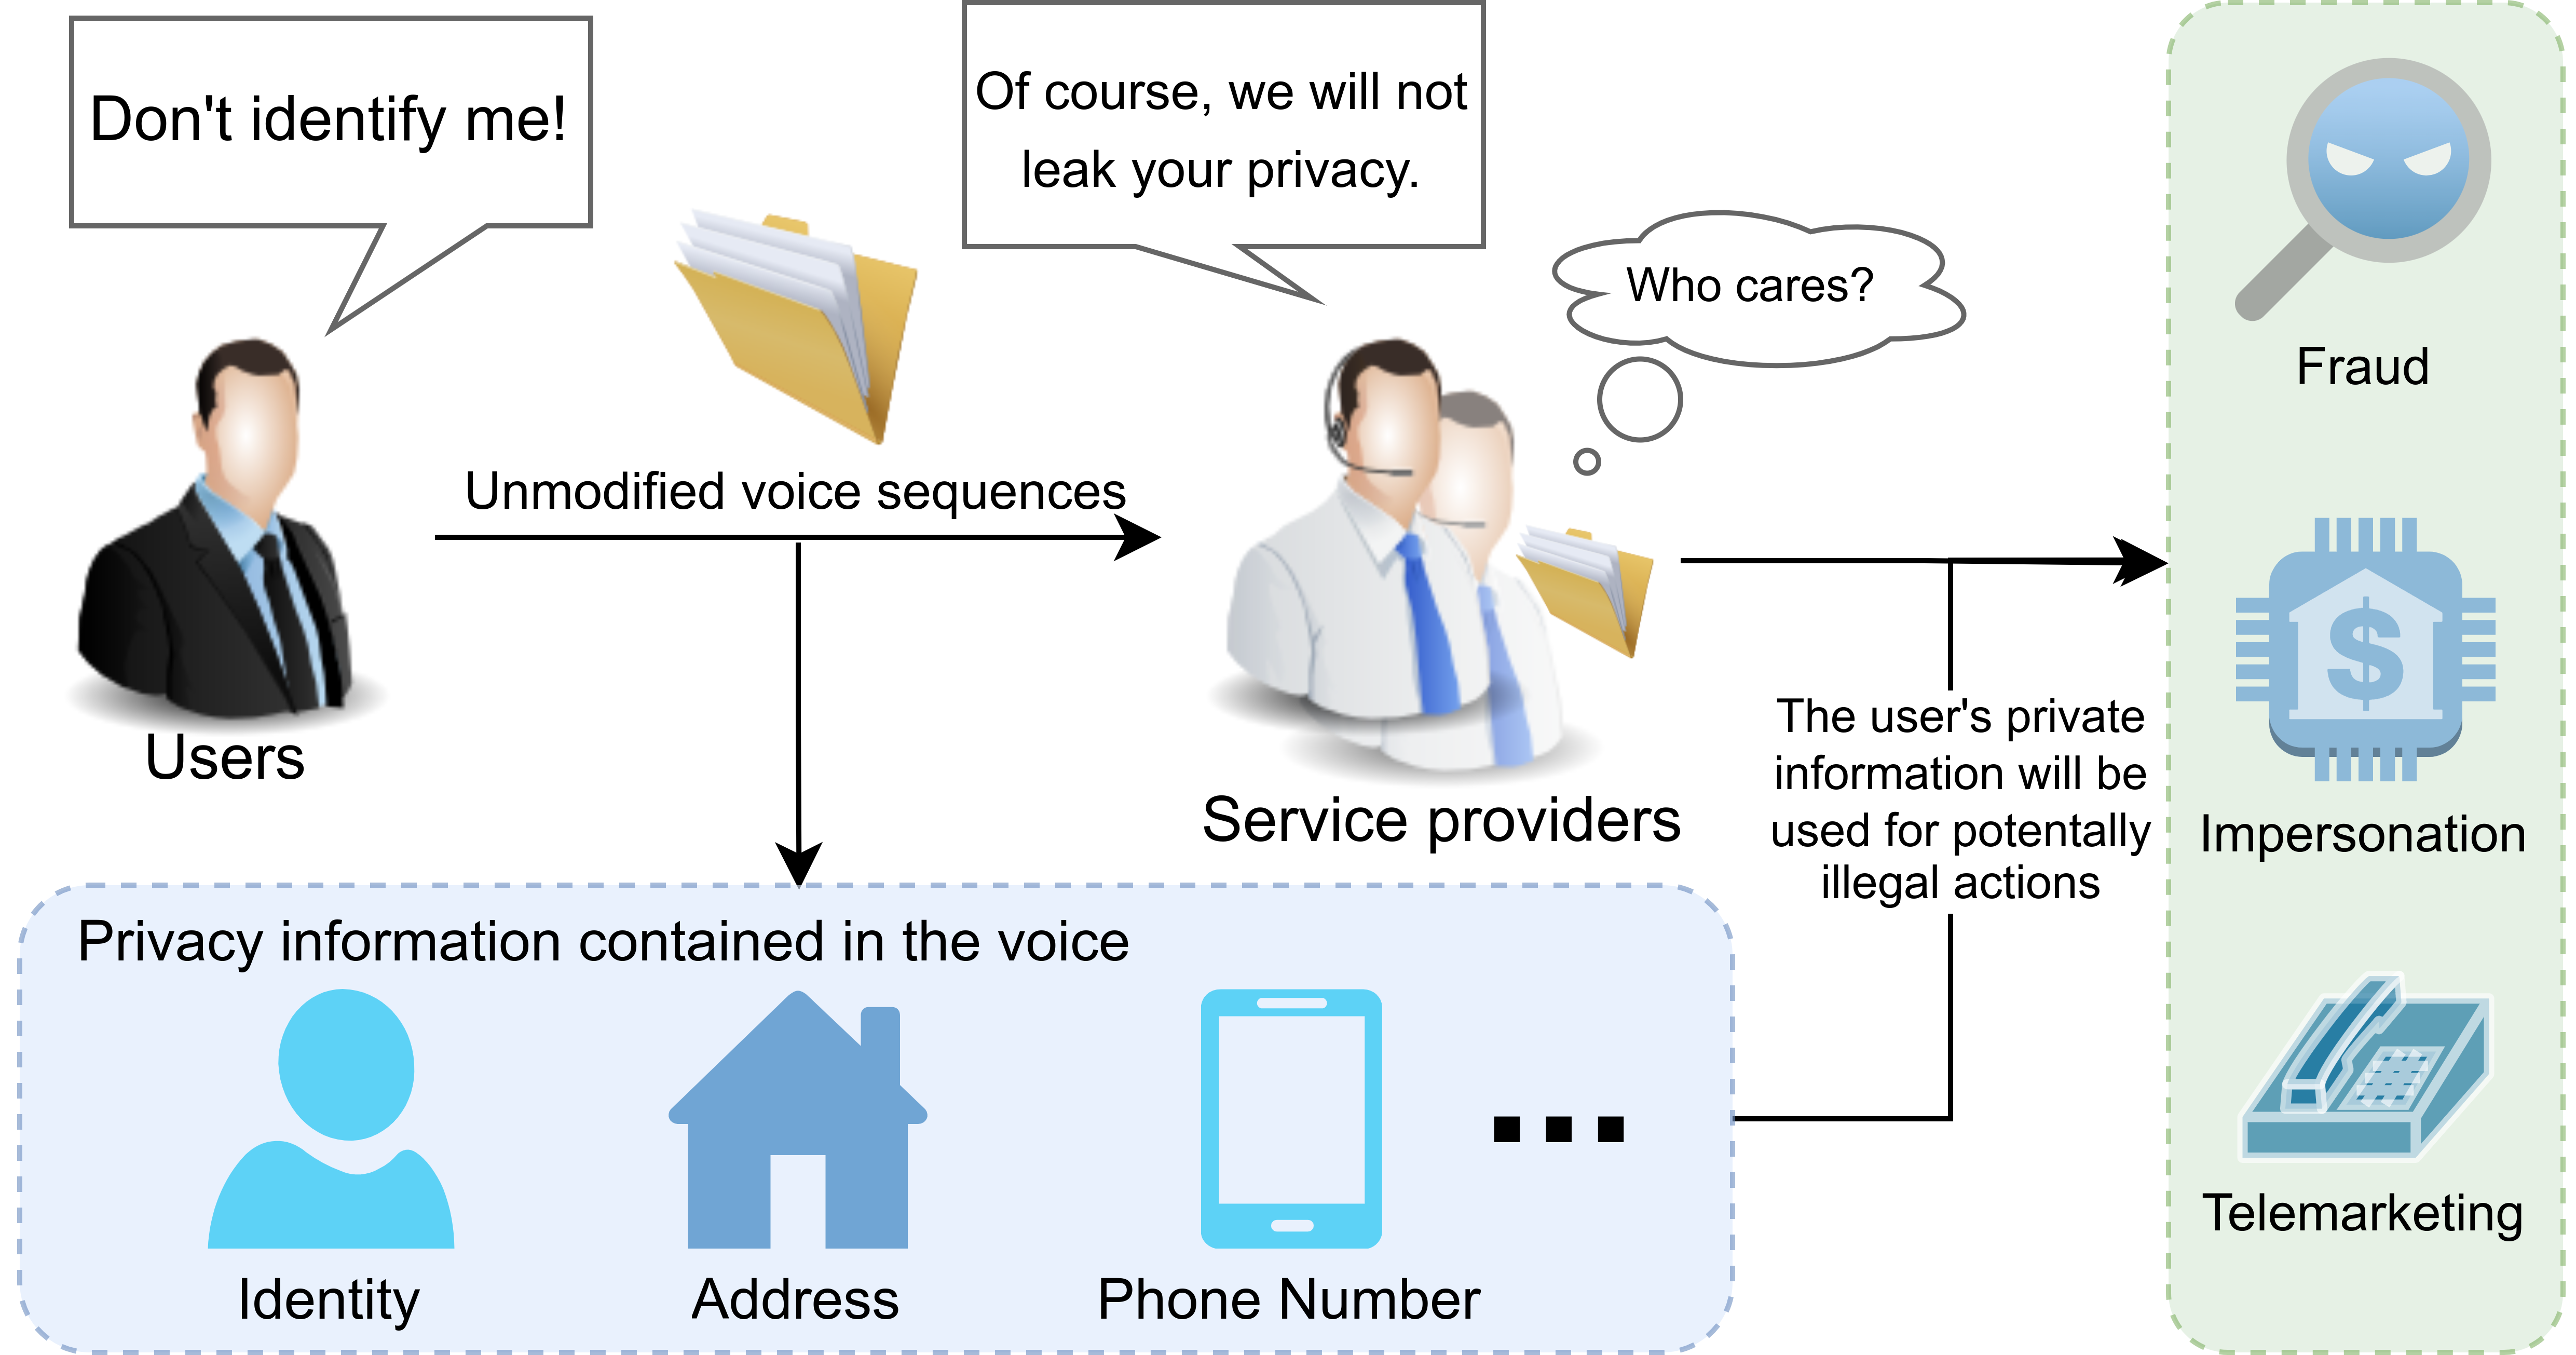
\includegraphics[width=2.5in]{case2v3.png}}
    \caption{Consequences of providing raw voice recordings with dishonest online speech service providers, from which it can be seen that this potentially leads to various types of malicious activities.}
    \label{fig:dishonest_provider}
\end{figure}

\begin{figure}[!t]
    \centering{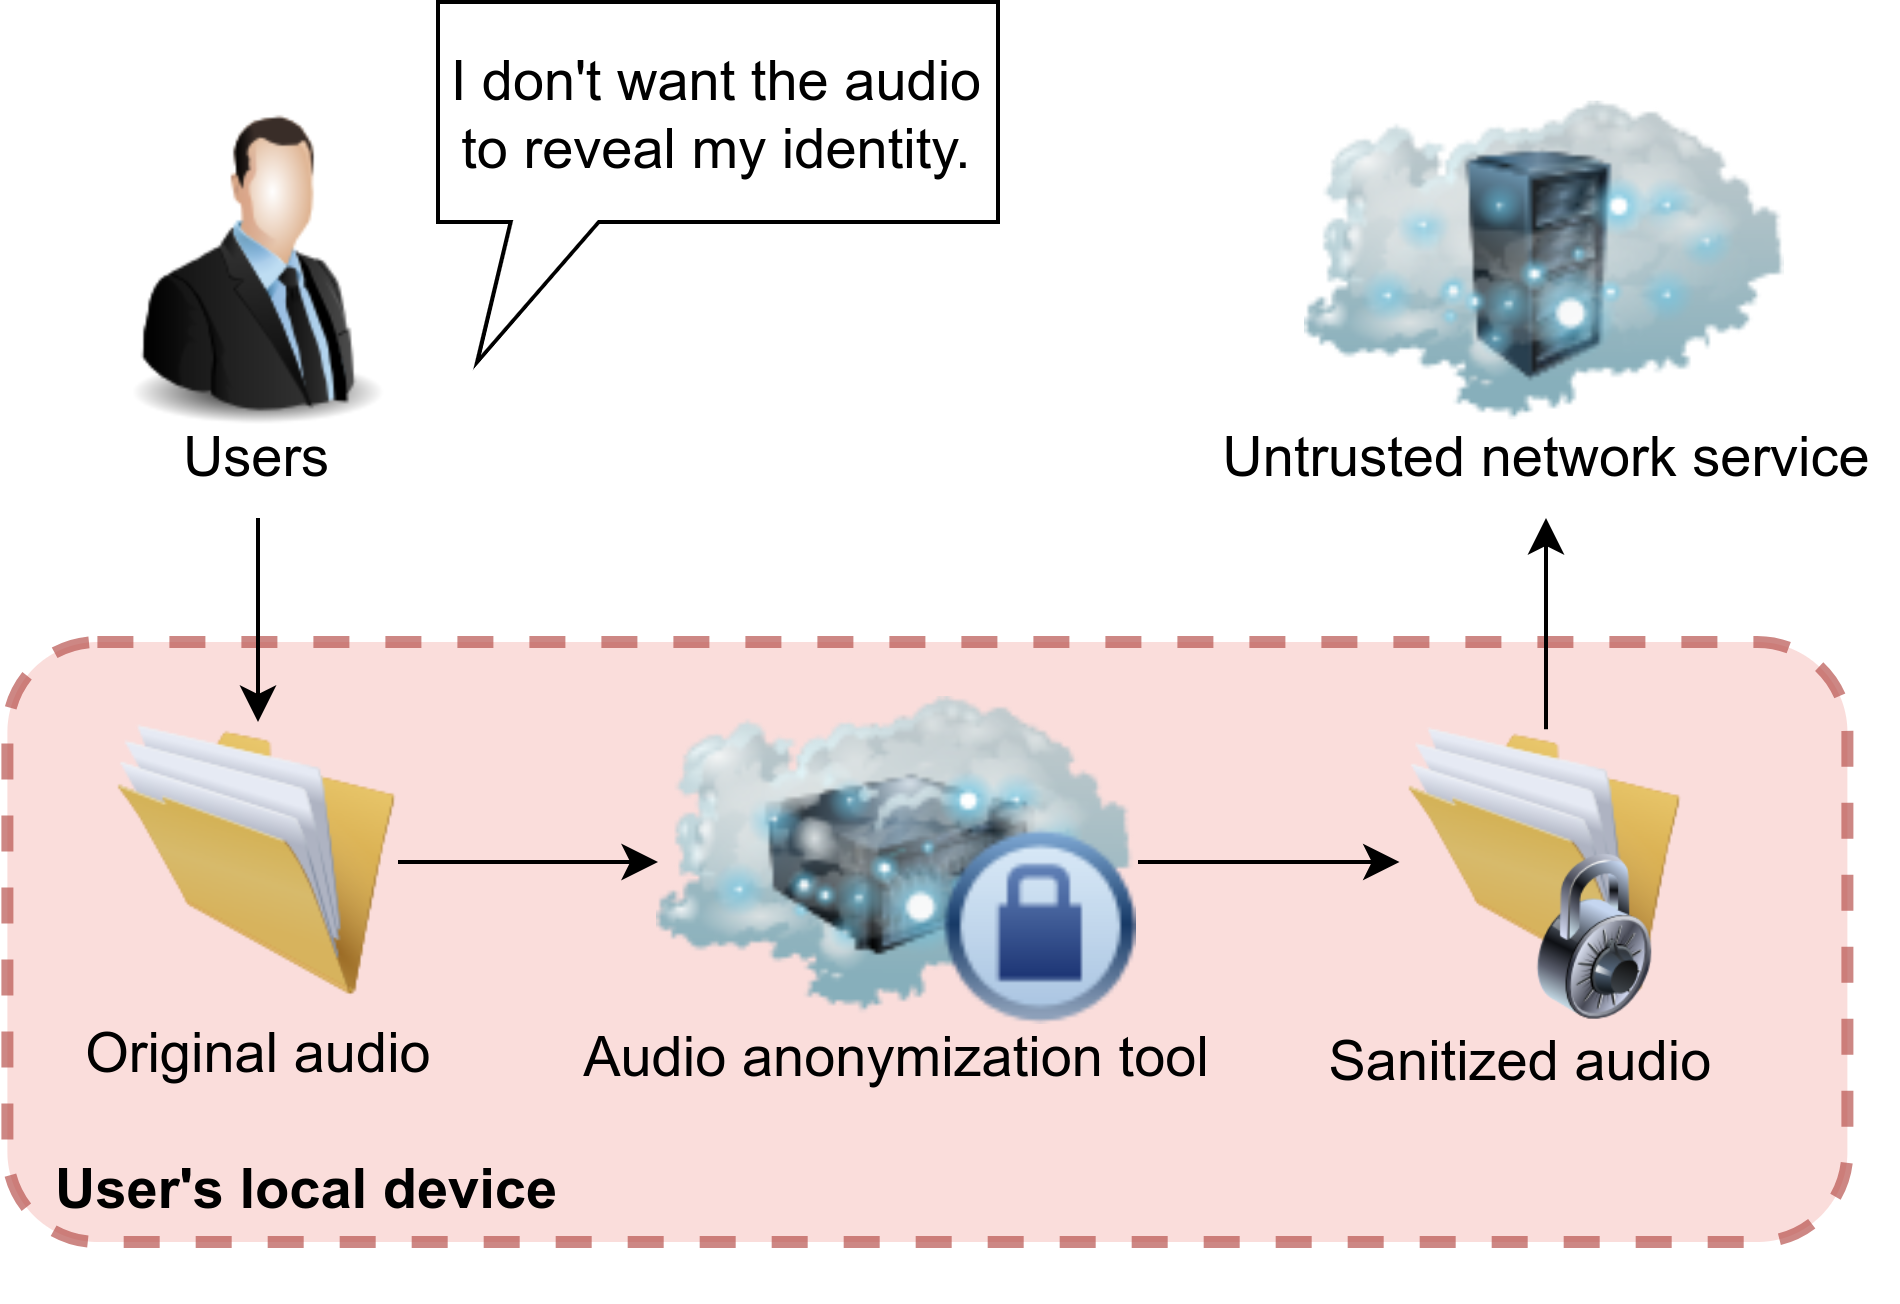
\includegraphics[width=2.5in]{case3v3.png}}
    \caption{The enforcement of voice deserialization by user. A specific \textit{Voice anonymization tool} is employed by the user, or by the service provider to meet user's security requirement.}
    \label{fig:privacy_enforcement}
\end{figure}

With the unprecedented abundance of large datasets and processing acceleration solutions, methods based on deep learning technologies has been enabled for a broad range of applications. Some voice-based services use voiceprint to prevent unwanted activations,such as Siri from Apple Inc.\footnote{https://www.apple.com/siri/} and Xiao Ai from Xiaomi Inc.\footnote{https://xiaoai.mi.com/}. Also, there are many voice enabled IMEs for various kinds of devices, such as iFly Input Method from iFlyTek\footnote{https://srf.xunfei.cn} and GBoard from Google, Inc.

However, what is also unprecedented is the ubiquity of such applications and services that raises novel privacy concerns. Provided the involvement of services that heavily use such personal data, recorded voice sequences, one has to take care to collect relevant data for services without inadvertently leaking sensitive information. Thus some technologies should be involved to safeguard user's privacy.

Consider a scenario where user wants to provide its voice recording, which is private, with an untrusted black-box application. If the original recording is provided untouched, it could result in the recording being used maliciously, as in Fig. \ref{fig:dishonest_provider} User alleviates such problem by using a third-party program or requiring the application to contain a module that remove sensitive information from the data (i. e. desensitize the data) while preserving the textual content and perform its own check to ensure the security, as described in Fig. \ref{fig:privacy_enforcement}

Researches are conducted regarding the privacy of voice recordings, which primarily focuses on two distinct areas: Removal of segments with sensitive textual content from the recording and the conversion of the voice sequence that replaces voiceprint, the vocal features of one speaker with another distinct set.

In this article we focus on the replacement of voiceprint and consider voice conversion the primary way to implement this type of desensitization. In this area StarGAN-VC is one of the state-of-the-art voice conversion algorithms, which is a deep learning model derived from the well known StarGAN, a many-to-many image style transformer model.

StarGAN-VC on its own could be considered as a valid desensitization algorithm. However, it focuses on the transformation performance and does not perform security measurements or tests in any way, which raises safety concerns. This brings us to the question that motivates us to this paper: \textit{Is voice conversion without further measures sufficient for desensitization of voice recordings?} In order to answer this question, we show that the desensitization results from a StarGAN-VC implementation can be used to embed with features from corresponding original recording, while ensuring minimum loss of quality and allowing the secret (i. e. original recording) to be extracted from it afterwards. From it, our results sound an alarm against the usage of data sanitization algorithms, and specifically StarGAN-VC, by third-parties. In summary, this paper makes the following contributions:

\begin{itemize}

\item We demonstrate the adversarial case: Hiding sensitive data in desensitized voice sequences.

\item We present its concrete workflow: a novel, adversarial exploitation of voice desensitization frameworks that.

\item We conduct experiments on a particular voice transformation model with well-known voice samples. From them, we analyzed the performance and potential of this attack framework.

\end{itemize}

The rest of the paper consists related works, an detailed explanation of the proposed methodology, including the discussion of potential use cases and opportunities of future works.

First we list and discuss related works on relevant topics in Section \ref{seg:related}. We then formulate our attack scenario to demonstrate our question previously mentioned with formal definitions in Section \ref{seg:problem}. Next, we describe the concrete implementation we set up for our experiments along with the design and metrics in Section \ref{seg:expriment}. After that the experiment results are analyzed and discussed in detail. The future work is discussed in Section \ref{seg:future} before concluding at the end in Section \ref{seg:conclusion}.

\section{Related work}
\label{seg:related}

\subsection{Adversary against desensitization}

There are researches on attacking privacy-preserving data transformation models. Some employ similar techniques that attempt to embed certain amount of data in sanitized data with modification to original deep-learning models and recover the original data after the exposure of sanitized data in public by victims. 

An notable instance among them works with images, targeting a privacy-preserving facial expression recognition algorithm, PPRL-VGAN. It sets up the attack with weak assumptions of user, who have white-box access to the attacked model. In order to achieve the adversary, its adversarial parts are embedded in the original model as additional layers or modification of existing layers, thus avoiding user's discovery.\cite{pprl-vgan,subvert}

However, there are much fewer works that propose adversaries against voice privacy preservation algorithms than facial image ones, even if the former is much more commonly adopted and deployed in production environment. The reason could involve the common misconception of voice-related technologies being mature or, even, complete.

\subsection{Voiceprint obfuscation}

Numerous research projects have been conducted for the preservation of voice privacy via the replacement of voiceprint. We consider these projects to fall in two categories: Traditional frequency-domain or voice tract analysis solutions and newer CNN-based voice transformation frameworks.

\subsubsection{Bilinear transform based methods}

Those employ frequency-domain analysis use various preprocessing techniques to deduce certain features from the raw voice sequences. Then a statistical formula is applied to obfuscate these frequency features. Reversing the preprocessing steps previously applied, the transformed voice sequences is obtained.\cite{a9, a10, a11}

These methods are more likely to suffer from the issues mentioned before that they are not able to complete cut the connections to the original voice sequences or erasing the relevant features, thus they are not further discussed in this paper.

\subsubsection{Deep learning based methods}

There also exhibits a number of solutions utilizing neural networks. These methods are more likely to employ less sophisticated preprocessing means and focus on increasing the complexity of CNNs. These methods benefit from recent improvements made on NN-based content generation algorithms and transformer frameworks, such as the Diffusion models commonly used with graphics data.\cite{a8}

However, also as mentioned before, these models are at times likely to be vulnerable to adversaries that utilize the non-significant part of a voice sequence, namely stenography algorithms. Lacking dedicated mitigation of such issues, it's possible to retain the crucial private data in a different form without user's notice.

\section{Problem statement}
\label{seg:problem}

\subsection{Assumptions}

The attacker has to use a form of stenography because it not only can not send the raw recordings over the network, but also may not have white-box access to the benign model to train or adjust for its purposes.

\subsection{Scenario}

\subsubsection{Users}

To users, the entire service is a black-box where they provide their raw voice sequences in exchange for services. Users can only verify the processed data that is actually sent to the remote servers.

\subsubsection{Attacker}

Attacker has access to a desensitization model to attack, either as a white-box with availability of source code or as a black-box with only public APIs. It want to modify this model or use another model as an add-in to embed features of original voice.

The only part where the attacker has access to raw sequences is the local program on user's device. Also, attacker has to ensure adequate difference between the raw sequences and the data sent to servers, which implies the recovery of original recordings is done remotely.

\subsection{Problem}

We consider the primary problem of our adversary generalizes to a specialized form of stenography where the desensitized sequence, as the carrier, carries the original counterpart the message. In this situation, the carrier and message share the same data type, format and textual content.

\subsection{Definitions}

In order to better formulate our methodology and implementation, we hereby formally define the following terms and their symbolic representations:

\begin{itemize}
    \item \textbf{Original voice sequence} $x$ is untouched voice recording from the user.
    \item \textbf{Desensitized voice sequence} $y$ is voice sequence processed by the sanitizer, with sensitive data removed.
    \item \textbf{Stenography embedded voice sequence} $y^{\prime}$ is $y$ with embedded information from $x$.
    \item \textbf{Extracted voice sequence} $x^{\prime}$ is the result of extracting $x$ from $y^{\prime}$ with embedded information.
    \item \textbf{Benign voice desensitization algorithm} $y = F_D(x)$ sanitizes $x$ into $y$.
    \item \textbf{Stenography embedding algorithm} $y^{\prime} = F_S(y, x)$ embeds features of $x$ into $y$ to get $y^{\prime}$.
    \item \textbf{Stenography extracting algorithm} $x^{\prime} = F_E(y^{\prime})$ extracts $x^{\prime}$ from $y^{\prime}$ according to embedded information.
\end{itemize}

\begin{figure}[!t]
    \centering{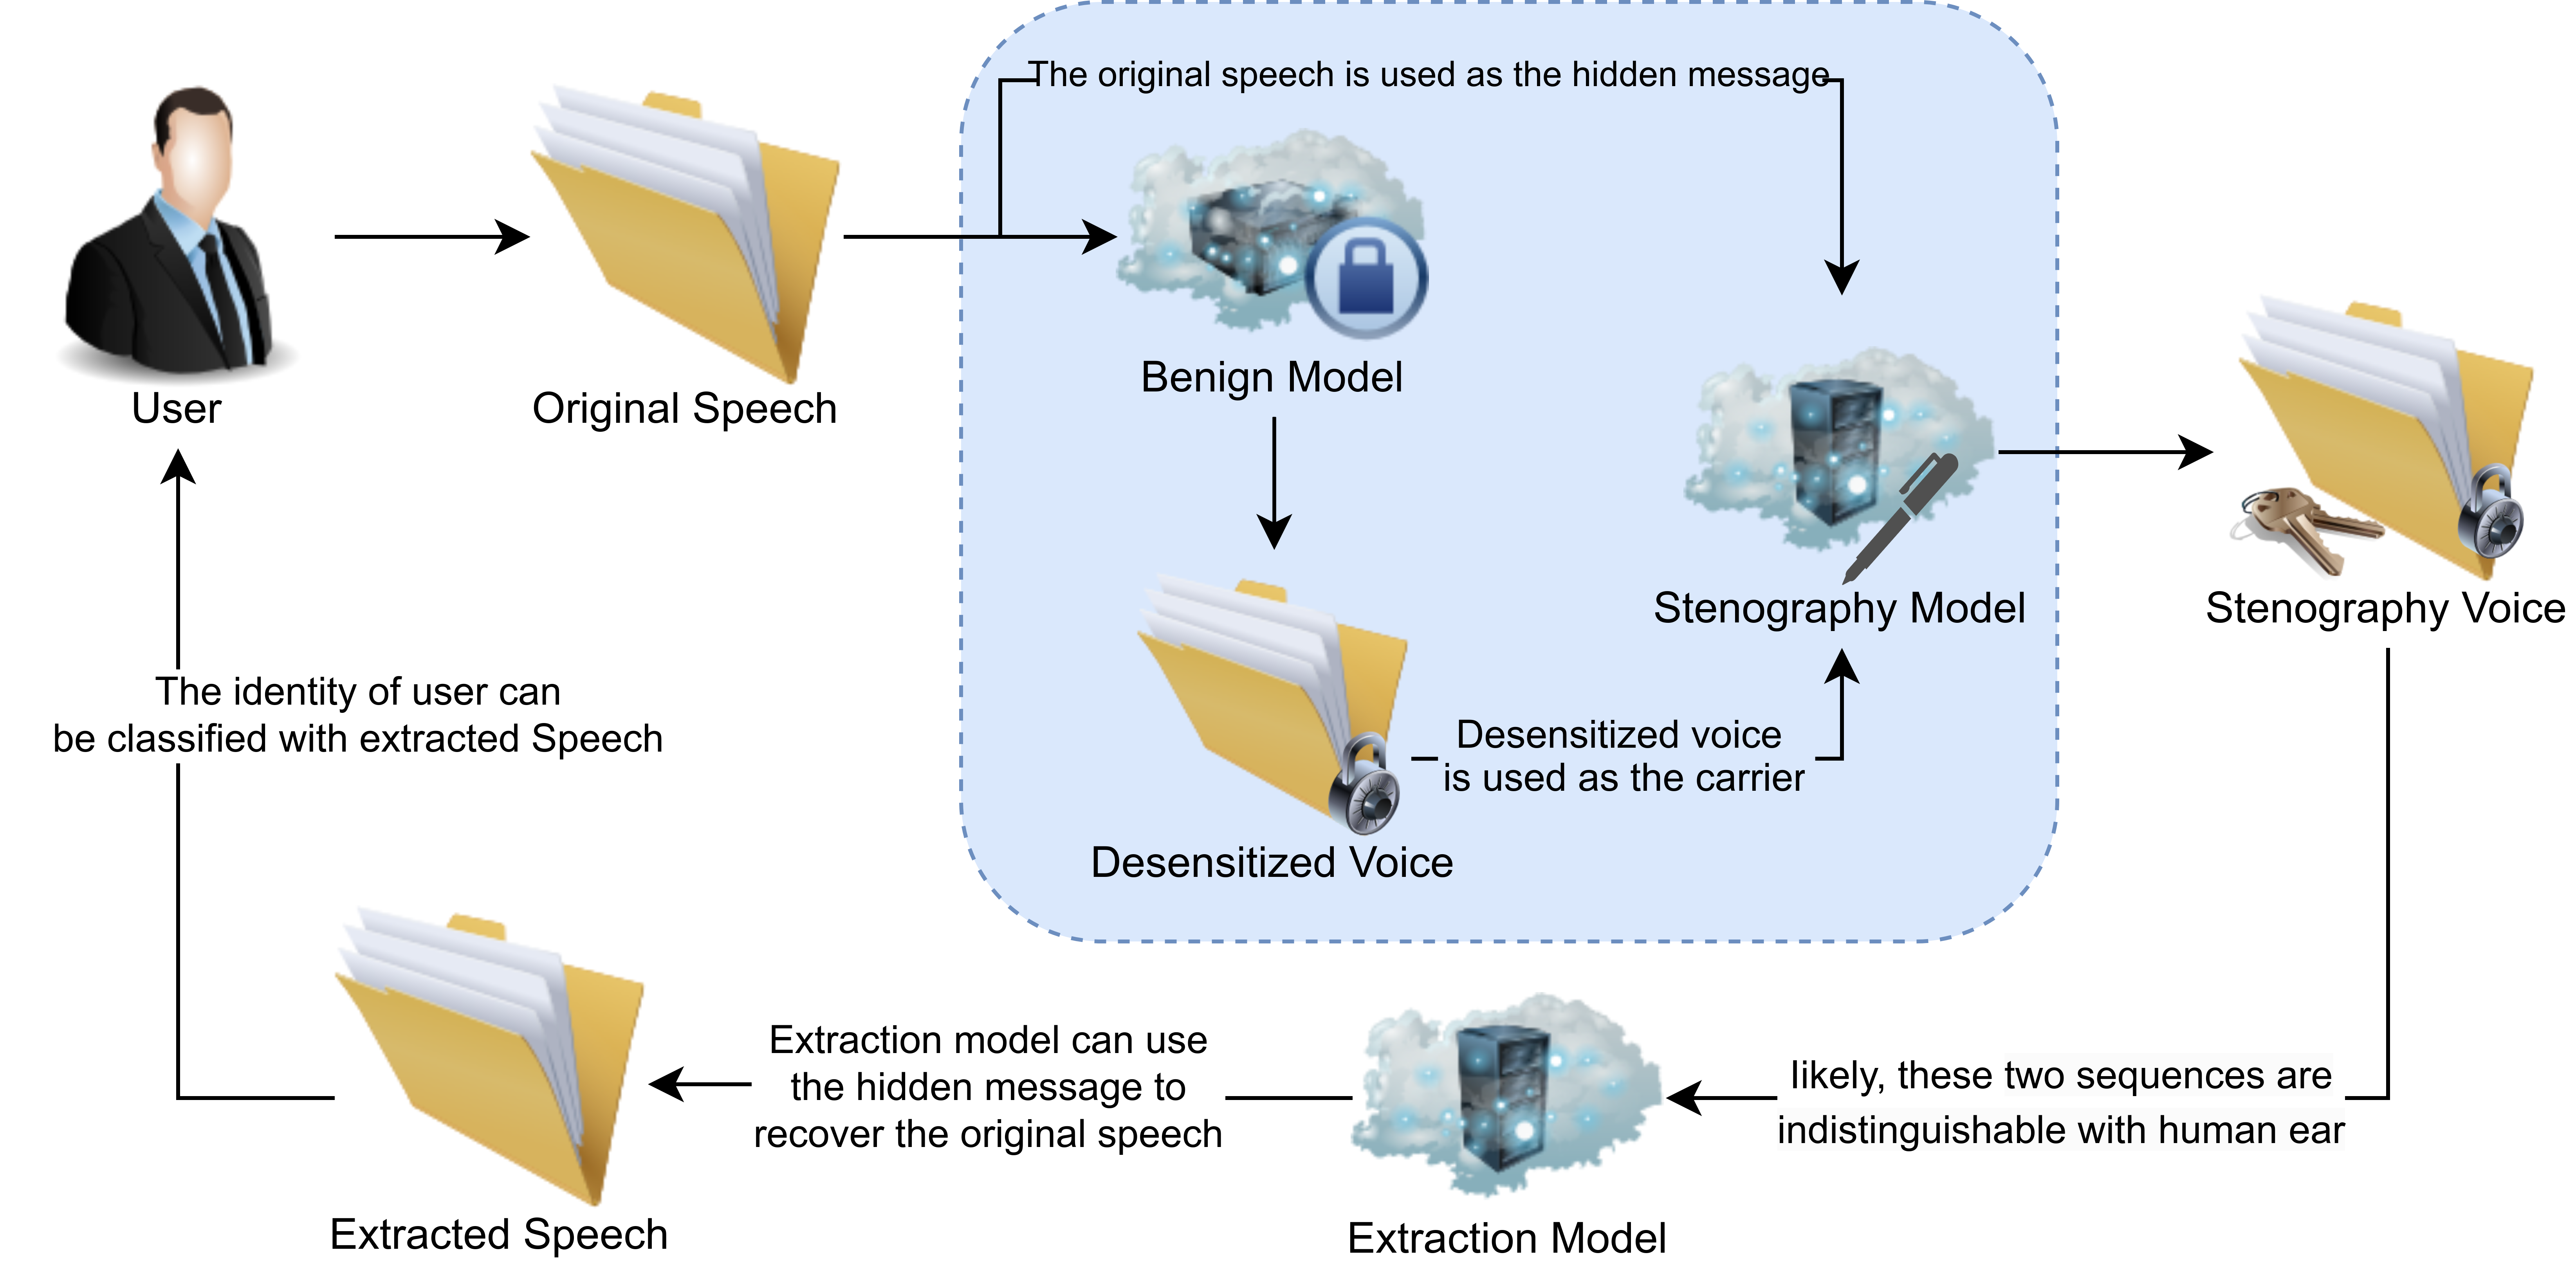
\includegraphics[width=2.5in]{methodv3.png}}
    \caption{The complete adversary workflow. Original voice recording $x$ is first processed by benign model $F_D$ into $y$. After that $x$ is stenographically embedded into $y$ to form $y^{\prime}$ by stenography (embedding) model $F_S$. After obtaining $y^{\prime}$ via the Internet, attack extract $x^{\prime}$ from $y^{\prime}$ via (stenography) extraction model $F_E$.}
    \label{fig:method}
\end{figure}

\section{Methodology}
\label{seg:method}

\subsection{Adversary Design}

\subsubsection{Desensitization}

The first step of our workflow, which is described in Fig. \ref{fig:method}, is to desensitize the original recording. Given $x$, $F_D$ is required to output $y$ that consists of distinct voiceprint than $x$ and identical textual content of it. One objective of StarGAN-VC\cite{a3}'s generator, the model we employed for $F_D$, is to generate plausible results that is not distinguishable from the real recordings. This ensures the integrity and structural correctness of generated voice sequence. It can be formulated as

\begin{equation}
    \label{eqn:adv_loss}
    \mathcal{L}_A = \mathbb{E}_{x}[\log D_S(x)] + \mathbb{E}_{x, c}[\log D_S(1 - G(x, c))]
\end{equation}

where $G(x, c)$ means the generated voice sequence from the authentic voice sample $x$ and the identity (i.e. label) of target speaker $c$ and $D_S(x)$ denotes the probability distribution provided by the discriminator $D_S$, which predicts the authenticity of its input. The value is minimized to deceive $D_S$. Another important objective is to generate results that closely resemble the target identity. This ensures when the supplied identity is a constant, as in our particular use case, the result will be identity-neutral, which is effectively sanitized from our standpoint. It can be formulated as

\begin{equation}
    \label{eqn:dom_loss}
    \mathcal{L}_D = - \mathbb{E}_{x, c}[\log p_C(c | G(x, c))]
\end{equation}

where $C$ is the domain classifier that predicts the speaker identity of one voice sequence. It takes a small value if $C$ correctly classifies $G(x, c)$, or $y$, into its target speaker identity. The value is thus minimized in order to improve the conversion performance.

As just mentioned, in our case the target identity is a constant $C$. In this way $F_D$ can be described as follows:

\begin{equation}
    \label{eqn:fd_val}
    F_D(x) = G(x, c)
\end{equation}

\subsubsection{Stenography embedding}

The next step is to embed features of original recording into the desensitized one. Given $y$ from the last step and $x$, $F_S$ is required to generate $y^{\prime}$ where sufficient amount of features of $x$ is embedded while maintaining high similarity with $y$. The primary goal of such stenography embedding model is described as

\begin{equation}
    \label{eqn:embed_loss}
    \mathcal{L}_S = \mathbb{E}_{x, y}[D(y, F_S(y, x))] + k\mathcal{L}_E
\end{equation}

where $D$ is general term for a function that calculate the distance between its parameters and $\mathcal{L}_E$ is the goal for stenography extracting mentioned below, where $k$ is a super-parameter that determines the balance between minimizing the modification made to the audio signal $(y^{\prime} - y)$ and the quality of extracted data $x^{\prime}$. The value is small when the similarity between the carrier, in which $x$ is written, and the stenography embedded $y^{\prime}$ (i.e. $F_S(y, x)$) is high. Thus, Hide and Speak, the deep-learning based algorithm we employed for $F_S$ in general optimizes for the minimum for it.

\subsubsection{Stenography extracting}

The final step after obtaining stenography embedded voice sequence is to extract the sensitive original recording from it. Given $y^{\prime}$ from the last step, $F_E$ is required to extract $x^{\prime}$ from it. The primary goal of such stenography extracting model can be described as follows:

\begin{equation}
    \label{eqn:extract_loss}
    \mathcal{L}_E = \mathbb{E}_{x, y}[D(x, F_E(F_S(y, x)))]
\end{equation}

The right hand side of this equation describes the distance between the original recording $x$ and the voice sequence extracted from $y^{\prime}$, which takes small value when $F_E$ provides sufficient information in $y^{\prime}$ to extract from and $F_S$ is of adequate quality such that the similarity between $x$ and its product (i.e. $F_E(F_S(y, x))$) is high. Both the stenography embedding and extracting algorithm optimizes for the minimum of this goal.

\subsection{Implementation}

\subsubsection{Benign desensitization model}

\begin{figure}[!t]
    \centering{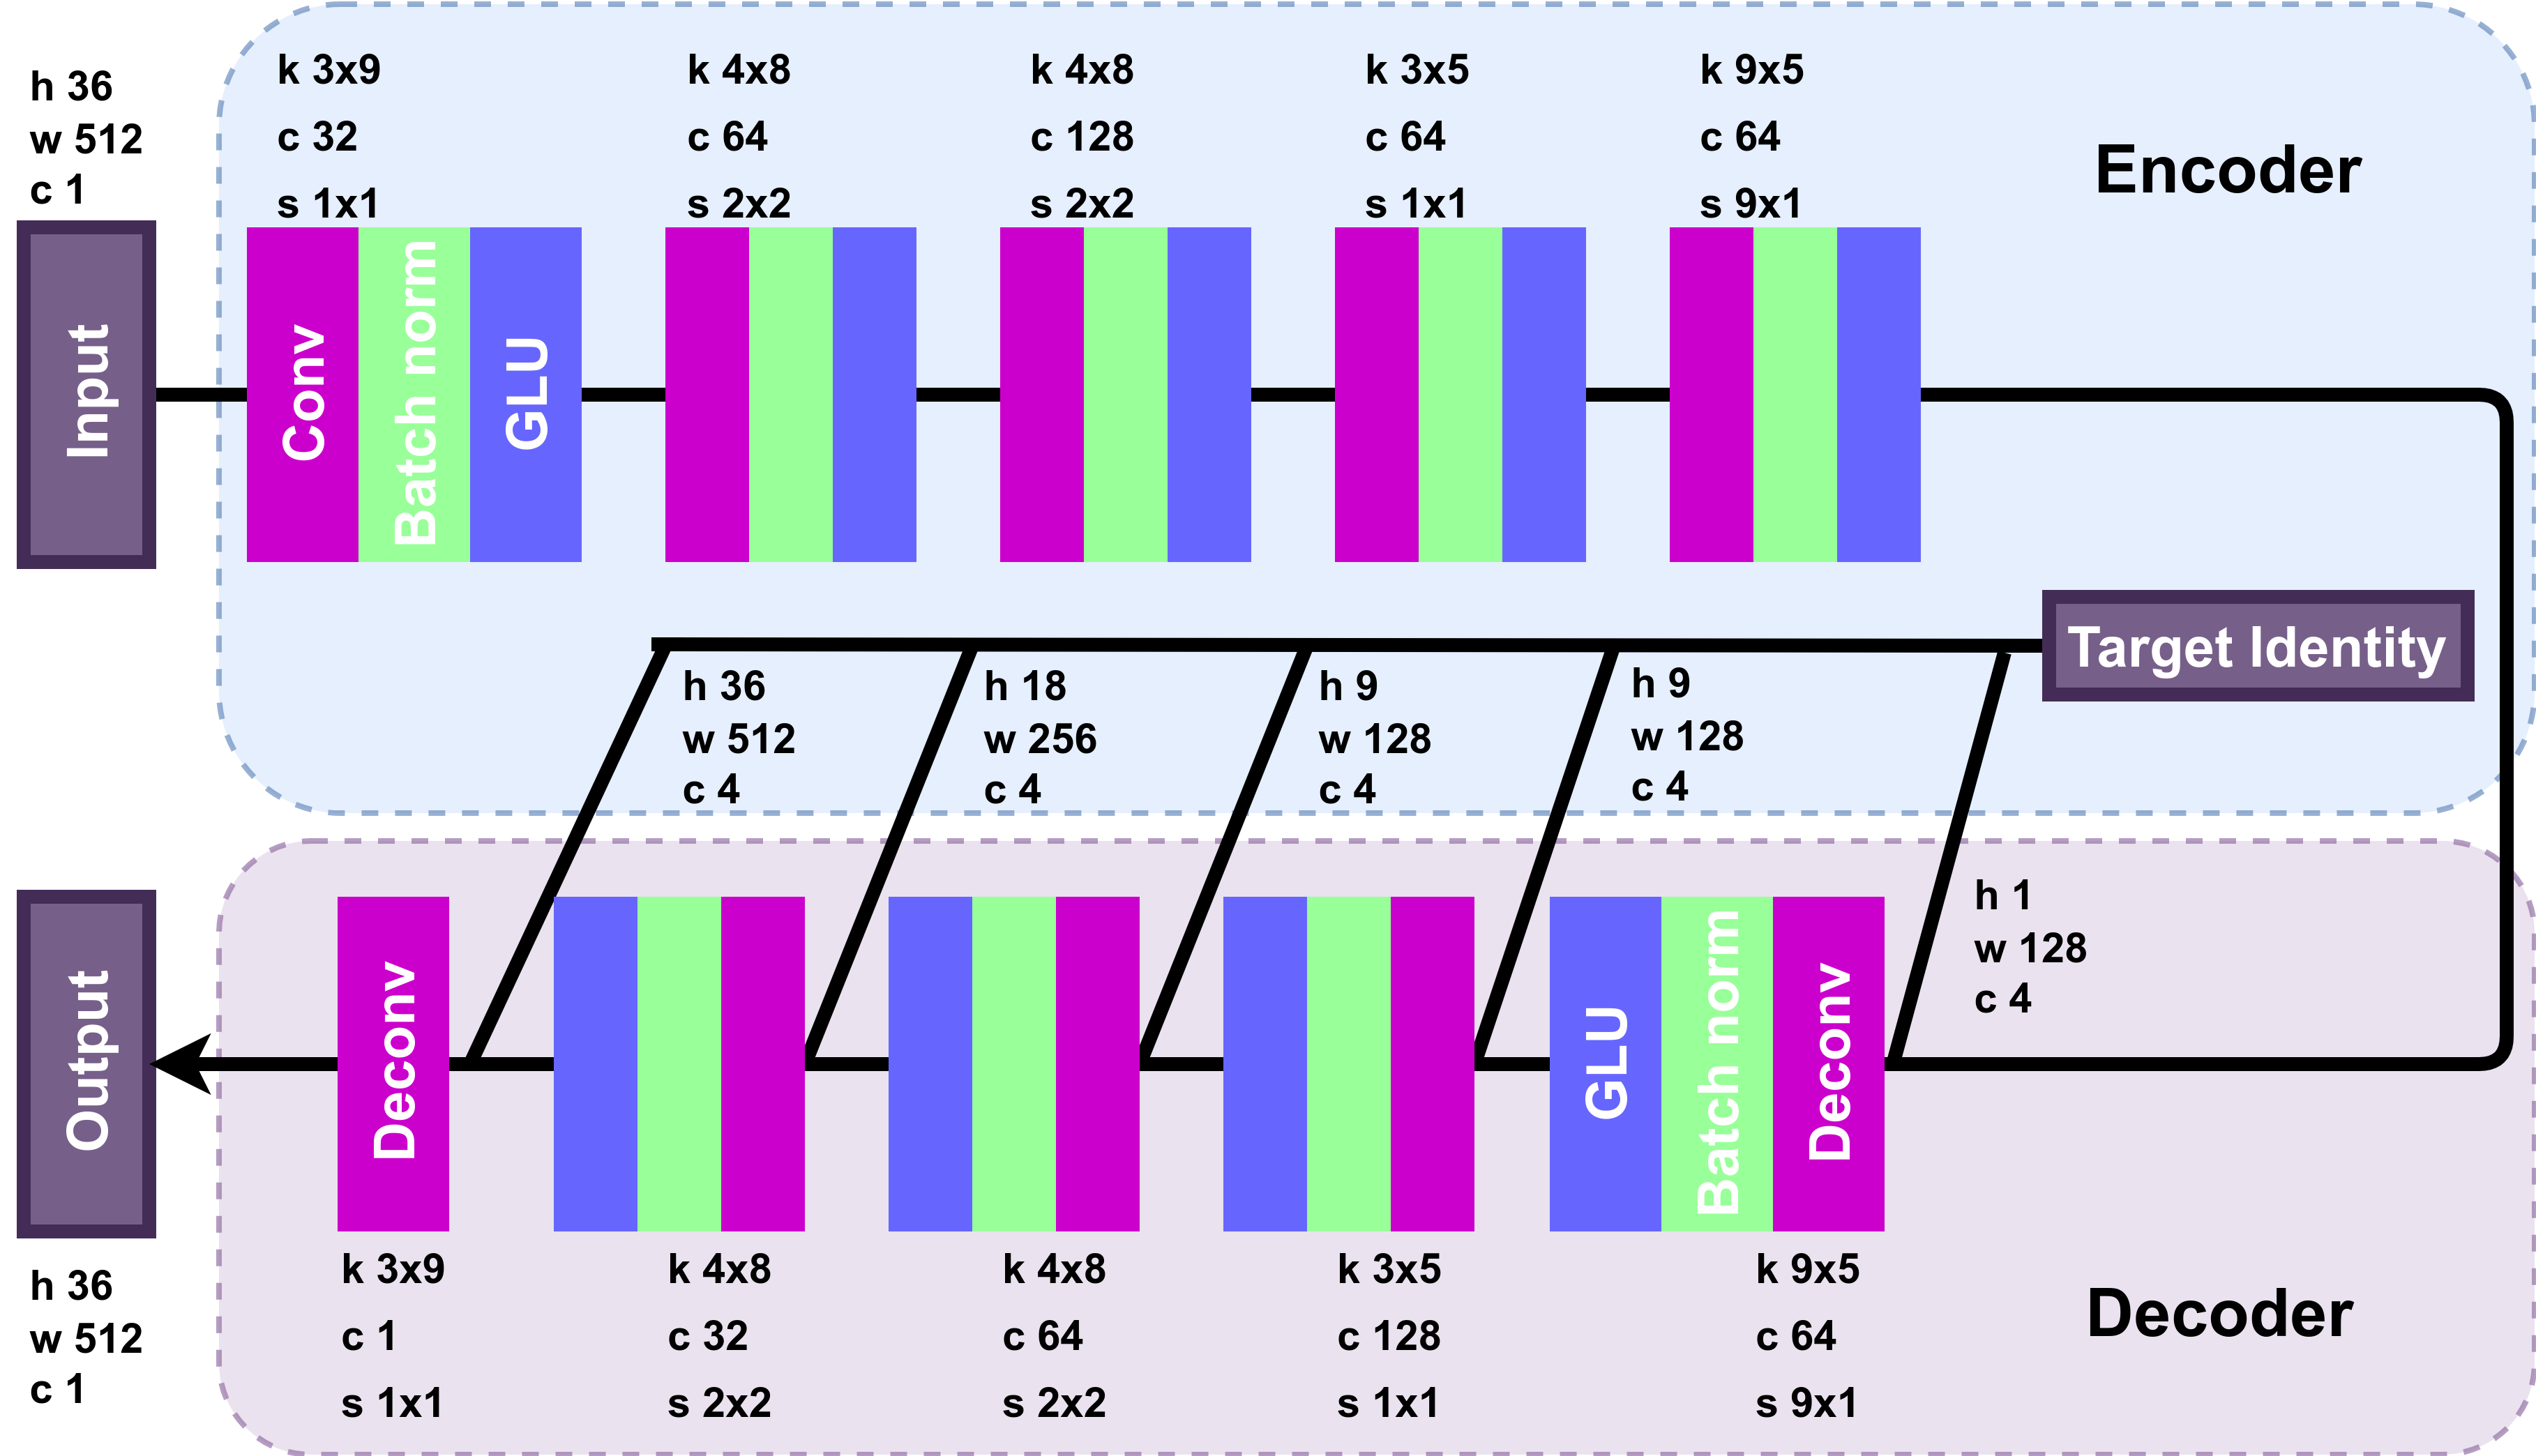
\includegraphics[width=2.5in]{struct_sgvc_model.png}}
    \caption{Structure of StarGAN-VC's generator, as $F_D$. Both the encoder and decoder parts consist of repeated combination of (de-)convolution layer, batch normalization layer and a GLU (Gated Linear Unit) layer. A layer made up of repeated speaker identity $c$ is stacked channel-wise before every set of decoder layers.}
    \label{fig:sgvc_impl}
\end{figure}

As mentioned previously, we use trained StarGAN-VC's Generator $G$ as $F_D$. The actual implementation of $G$ we employed for experiments closely resembles the official implementation, as depicted in Fig. \ref{fig:sgvc_impl}, where $x$ is first processed by a series of convolution layers, as a decoder, in order to extract its textual speech content. After that, a layer of repeated $c$, which is the target speaker identity, is stacked channel-wise against the intermediaries of every further layers, as the decoding part. Since instances of $x$ are variable length by nature and $G$ accepts fixed-sized input, they are split into segments (and zero padded) as a step of preprocessing.

\subsubsection{Stenography models}

\begin{figure}[!t]
    \centering{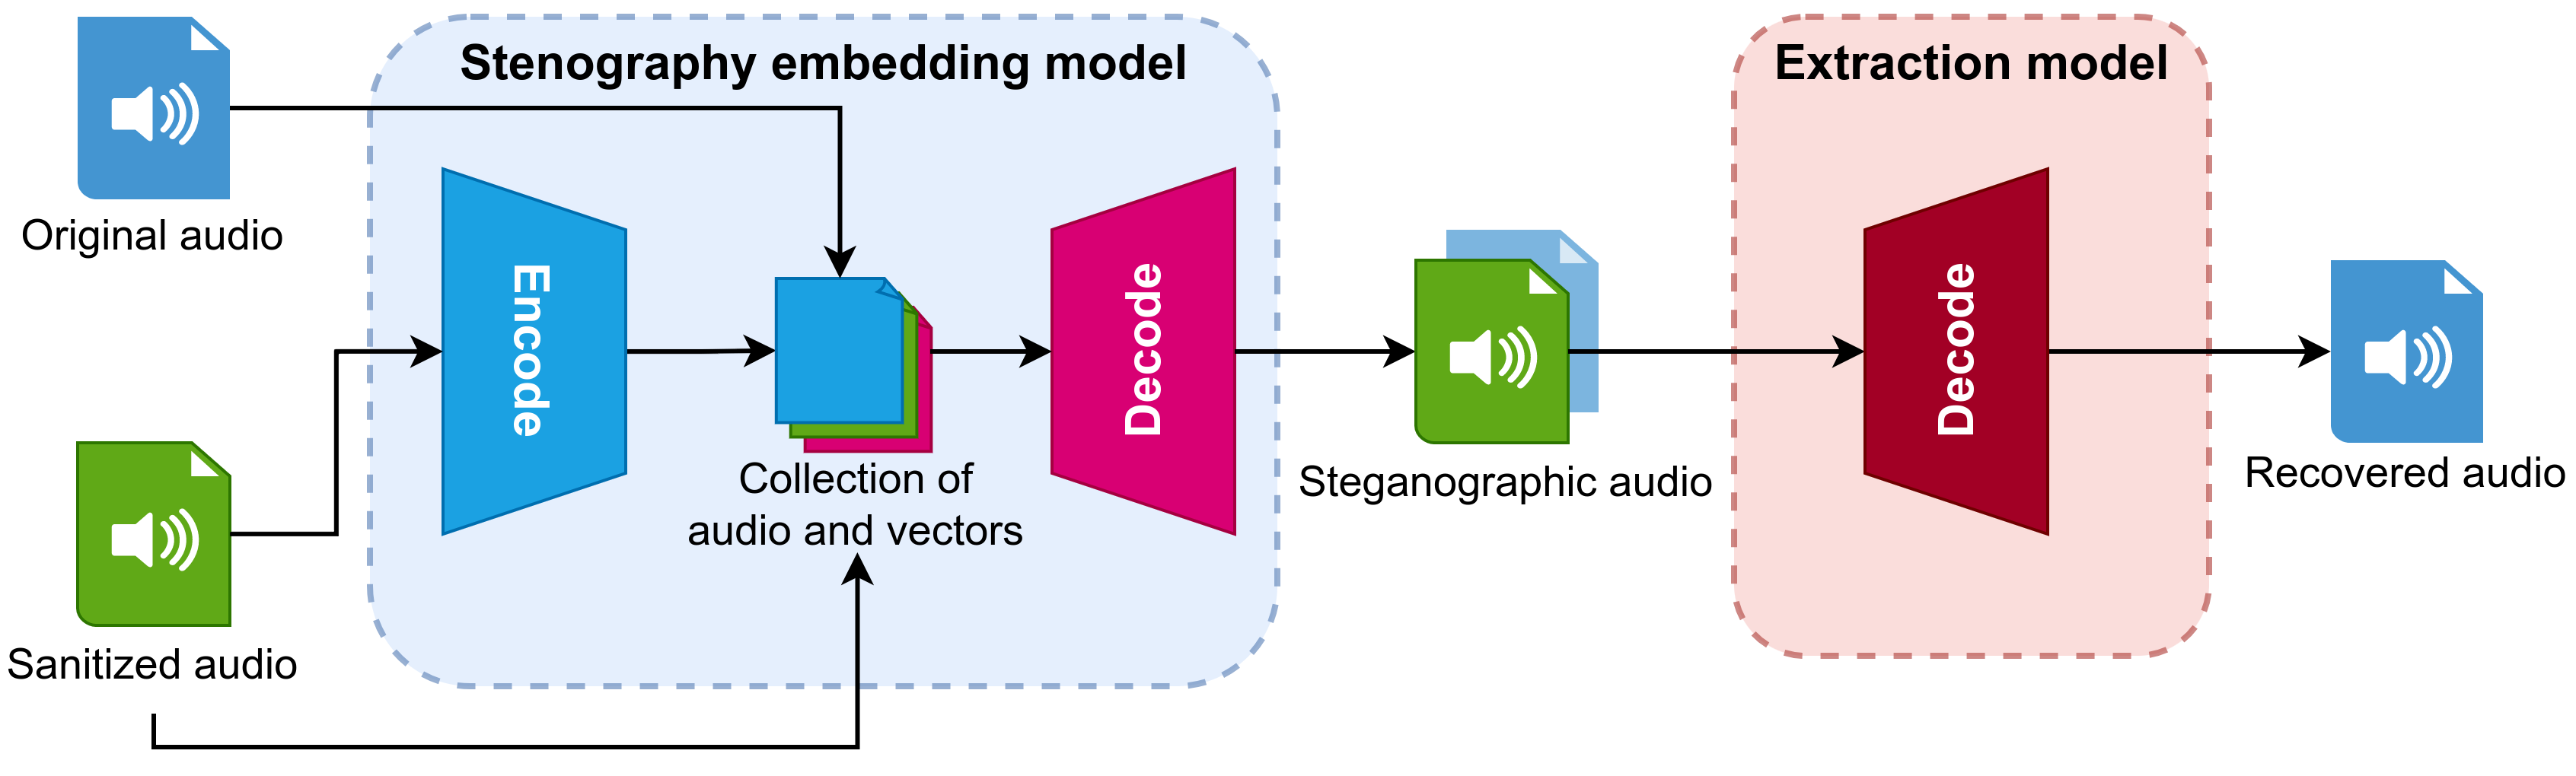
\includegraphics[width=2.5in]{struct_steno_models.png}}
    \caption{Structure of stenography embedding (as $F_S$) and extraction (as $F_E$) models where the conversion between magnitude and time-domain representation is not shown. A hybrid representation of $x$, $y$ and latent representation of $y$ generated by \textit{Encode} part of stenography embedding model is used.}
    \label{fig:steno_impl}
\end{figure}

Also mentioned before, $F_S$ and $F_E$ are provided by Hide and Speak's stenography embedding and extracting models. Here we used the official implementation, as depicted in Fig. \ref{fig:steno_impl}, where for $F_S$ a joint representation of secret message $x$ and stenographic carrier $y$ is created with additional latent information from an carrier encoder network. Then, this representation acts as the input of carrier decoding network, which outputs the magnitude representation. This is then converted into time-domain signal (i.e. $y^{\prime}$). For $F_E$, $y^{\prime}$ is first converted back into magnitude representation before being processed by message decoder network, into extracted original recording $x^{\prime}$.

\section{Experiment}
\label{seg:expriment}

Recall our workflow, where user produces voice recordings for certain services, and it's processed by attacker's adversarial desensitization service and finally, the original sequence is extracted from the desensitized one in the cloud. In order to closely approximate such process and evaluate the effectiveness and versatility of our workflow, we conducted the following experiment.

\subsection{Setup}

\subsubsection{Dataset}

\textit{VCC 2016} dataset, where VCC means Voice Conversion Challenge, which is what it was designed for, is employed for training of $F_D$ and generation of data for our evaluation. In this dataset there are 10 speakers including 5 male and 5 female ones. Each speaker has the same number of voice samples (162 for training and 54 for evaluation) where the corresponding textual content of each one across every speaker remains the same. Each voice sample are down-sampled to 16 KHz from the DAPS (Device and Produced Speech) dataset. However, their length and clarity is not guaranteed to be the same. In order to keep the experiment straightforward, only four speakers, SF1-2, TM1-2 are chosen for training.

\textit{TIMIT} dataset, The DARPA(Defense Advanced Research Projects Agency) TI(Texas Instruments)MIT(Massachusetts Institute of Technology) Acoustic-Phonetic Continuous Speech Corpus, which consists of 6300 recordings of spoken sentences by 8 different dialect regions of the U.S, is used for the training of $F_S$ and $F_E$. The diversity and quantity of this dataset helps with the versatility of Hide and Speak model in terms of voice processing.

\subsubsection{Preparation}

As implied previously, our workflow requires three distinct models, benign desensitization model for $F_D$, stenography embedding model for $F_S$ and the extraction one for $F_E$. As part of the experiment preparation, we trained these models according the methodologies described in previous sections, where the benign model is trained for 200000 steps with VCC 2016 dataset and the stenography model and extraction model are trained with TIMIT dataset.

Our workflow accepts user's raw voice sequences, $x$, as input, as described before. In our experiment, we substitute this with both training and evaluation dataset of VCC 2016 dataset, which closely resembles this use case. In this way, we got 648 samples in total from 4 speakers where each has 162 samples. It's worthwhile to mention that we consider the usage of training data in our experiment where the same data is used for training of the benign model legit because of the fact that the generalization ability of our voice transformation model is not the most important concern. Even the benign model naturally performs better on its training set, our experiment focus on the effectiveness of the overall workflow instead of individual performance of its parts.

\subsubsection{Generation}

It's easy to notice that the complete workflow produces 3 distinct products, along with the original recording forms a set of 4 voice sequences for each sample, $x$, $y$, $y^{\prime}$ and $x^{\prime}$. All of these voice sequences are included in our experiments. Since each sample can be used to generate 3 sets of voice sequences targeting different speakers, we get 1944 sets in total.

\subsection{Design}

\subsubsection{Voiceprint Recognition}

The success or failure of our adversary, of which the goal is to acquire user's identity after desensitization, can be determined by measuring the performance of voiceprint recognition services on the extracted original voice samples. Additionally, the impact of stenography can also be measured in this way.

For this experiment, we employ a high-performance cloud-based voiceprint recognition solution from iFlyTek that takes in the voice samples and generates results for each samples that contain likelihood scores for each speaker varying from 0 to 1. Higher scores mean greater possibility that a voice sample belongs to a particular speaker. According to the official documentation, an score

\subsubsection{ABX Test}

Though our voice samples and results are not exactly intended to be taken by human ears, it's useful to ensure that the desensitized voice samples do not sound like the original ones and the recovered ones are intelligible. In this case, we conduct ABX test, where given original samples of each speaker, participants identify the class of random choices of voice sequences, on numerous subjects. Notice that our ABX experiment does not strictly conforms to the definitions since we have 4 categories instead of 2 and the test samples do not strictly belong to the original recordings. However, the set of speakers are the same.

The type of recording played, which is one variant in the tuple mentioned in our setup, the original speaker and what the participant chose is stored as one record for analysis. Additionally, the file name of recordings are stored and target information of desensitization process can de deduced from it.

\subsubsection{Metrics}

There are over 2000 numbers in the result of voiceprint recognition experiment. In order to organize them in an intuitive manner, we calculate following statistical values from them, respectively for every kind of speech sequences and each speaker:

\begin{itemize}
    \item \textbf{Mean} - Average value of scores. Higher values mean generally closer to the original speaker.
    \item \textbf{Certainty} - Ratio of scores being greater than 0.6, which means the sample can be confirmed to bear the same speaker as the original one. Higher values mean values are more definite.
    \item \textbf{Best} - Best value of scores.
    \item \textbf{Worst} - Worst value of scores. Closer value with \textbf{Best} means better stability.
    \item \textbf{Class Ratio (Abbreviated as "Class R.")} - Ratio of samples being classified into its original speaker, i.e. have the highest score being the original speaker, as mentioned before. Higher values mean higher probability an generic classification model will think the samples have the same identity of the original speakers.
\end{itemize}

As for the ABX test, we derive the following statistics from our records in order to present clear cut results:

\begin{itemize}
    \item \textbf{Degradation (Carrier)} - Decrease of correct rate of detecting the carrier's identity from desensitized samples to stenography ones.
    \item \textbf{Degradation (Message)} - Decrease of correct rate from original samples to extracted ones.
    \item \textbf{Conversion (Target)} - Rate of participants recognizing the target identity of converted samples (desensitized and stenography ones).
    \item \textbf{Conversion (Phantom)} - Rate of recognizing the \textbf{original} identity of samples just mentioned.
    \item \textbf{Gender (Vague)} - Rate of choosing a identity of the same gender as the identity of a sample.
    \item \textbf{Gender (Exact)} - Rate of choosing the exact identity of a sample.
\end{itemize}

\subsection{Results}

\begin{figure*}[tb]
    \centering{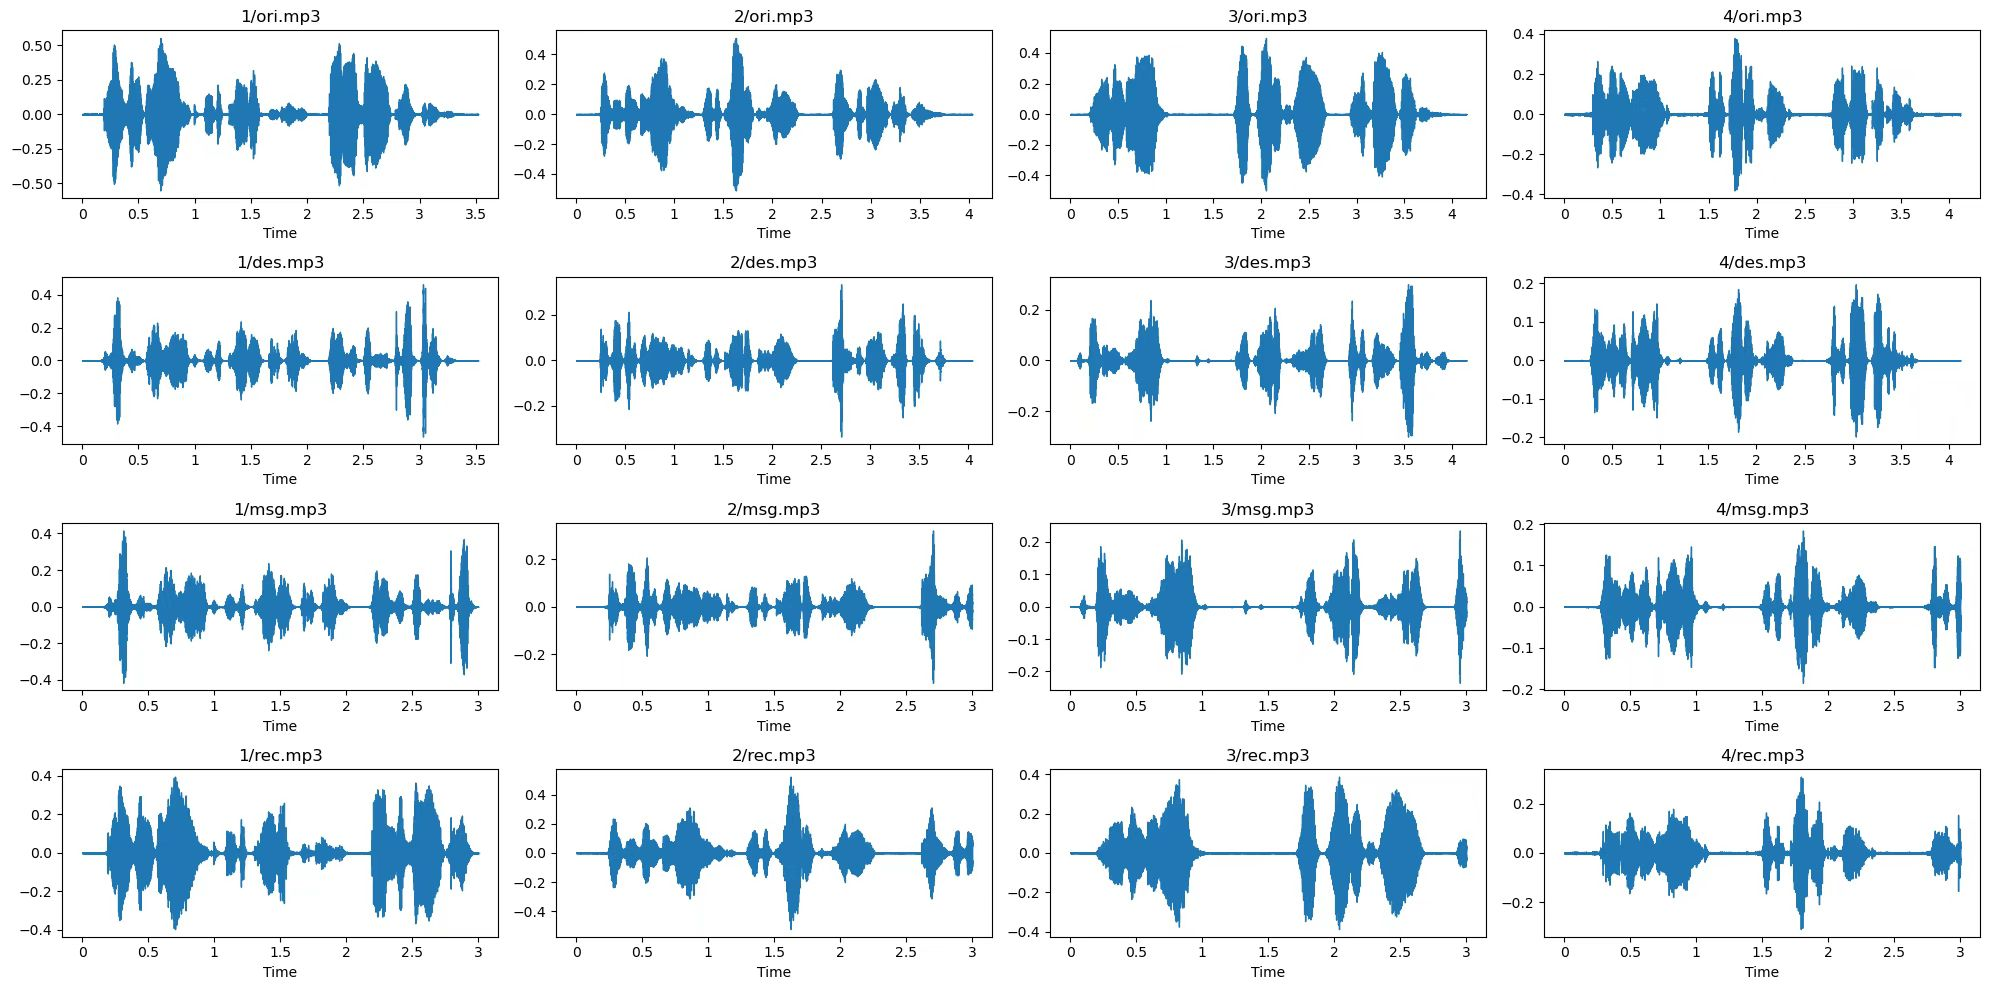
\includegraphics[width=\textwidth]{samp_wav.jpg}}
    \caption{4 samples. Each column from top to bottom contains corresponding waveform of $x$ as \textit{ori}, $y$ as \textit{des}, $y^{\prime}$ as \textit{msg} and $x^{\prime}$ as \textit{rec}. It can be seen that $x^{\prime}$ is sufficiently similar with $x$, which can be consider as an indication of the success of adversary.}
    \label{samp1}
\end{figure*}

What is depicted in Fig. \ref{samp1} is 4 sets of voice samples in different stages of processing, from which it's noticeable that the overall performance of this adversary is reasonable. Fig. \ref{chart_mean} displays the overall mean scores.

\subsubsection{Original samples}

According to Table I, all of the score statistics, except for the \textbf{Worst}, are close to 1, which is intended behavior for original samples. As the worst case, \textbf{Worst} is also close or greater than 0.6, which means that even this type of cases are confirmed to have the same identity as the original speaker. As a result, it's safe to confirm that both the benign model and the validation service are of desirable performance.

\subsubsection{Desensitized samples}

According to Table II, the overall score dropped drastically from over 0.8 to over 0.4. It can be argued that from the \textbf{Best} and \textbf{Class Ratio} numbers that there still exhibits a portion of samples that are classified into the original speaker. However, these type of classification results can not be trusted because they are vague, according to the close-to-zero \textbf{Certainty} value.

\subsubsection{Stenography samples}

Scores of stenography samples are similar to the desensitized ones, given the numerical changes of statistical numbers are mostly less than 0.1. However, the changes stenography model made to the samples did not cause any form of degradation of desensitization performance, but upgraded it instead.

Table V is the statistics of direct comparison between these two sets of samples. According to the \textbf{Minimum} value, it's still possible that the desensitization performance would suffer significant degradation from the stenography process, but from the \textbf{Mean} and \textbf{Variance} value we can see that the performance changes are even-spread.

It's highly likely that the changes are caused by the slight content degradation, i.e. perturbation, made by stenography model and would not strongly affect the overall performance of such adversary. We also performed manual audio quality tests on a random subset of this set of samples and confirmed that the degradation is not audible.

\subsubsection{Extracted samples}

As mentioned before, extracted samples are meant to be as close to the original samples as possible. As presented in Table IV, the values are slightly inferior than the original samples with the decrease of score within 0.1 to 0.2. However, despite the worsen results, the \textbf{Certainty} and \textbf{Class Ratio} are still well desirable, suggesting that the usability of these samples are comparable to the original ones, which declares the success of adversary.

\subsubsection{ABX Test}

Fig. \ref{fig:degradation}, where the audible degradation of carrier varies from -0.2 to -0.3, indicates the inevitable reduction of audio clarity after stenography operation. However in the same figure it's clear that the audibility of message, what stenography model embeds in the carrier, suffers far less damage. To a certain degree the clarity actually increased in the extracted sequences, which may be contributed by the voice-optimized nature of such method.

Fig. \ref{fig:transform} indicates that the performance of participants recognizing the target identities of desensitized (i.e. converted) samples varies from none to over 50\% accuracy. However, every participant have a slight possibility of choosing (accidentally or purposefully) the original speaker of a converted sample with two of them have a non-negligible over 30\% accuracy. We consulted with these subjects and confirmed that there are slight ghosting effect in converted samples that is human-recognizable. However, it is too slight for recognition models to confirm as its identity.

Additionally, we analyzed Fig. \ref{fig:gender} due to a degree of similarity between two female speakers (SF1-2)and male speakers (TM1-2). What is depicted in the figure shows that There is a case where the participants mix the speakers of the same gender. This case is not significant, however.

\begin{table}[!t]
    \centering
    \caption{Statistics of Original Samples}
    \begin{tabular}{|c|c|c|c|c|c|}
        \hline
        & \textbf{SF1} & \textbf{SF2} & \textbf{TM1} & \textbf{TM2} & \textbf{Mean} \\
        \hline
        \textbf{Mean} & 0.853889 & 0.837284 & 0.84537 & 0.837963 & 0.843627 \\
        \hline
        \textbf{Certainty} & 1.0 & 0.987654 & 1.0 & 1.0 & 0.996914 \\
        \hline
        \textbf{Best} & 0.95 & 0.94 & 0.94 & 0.94 & 0.9425\\
        \hline
        \textbf{Worst} & 0.6 & 0.56 & 0.6 & 0.61 & 0.5925\\
        \hline
        \textbf{Class R.} & 1.0 & 1.0 & 1.0 & 1.0 & 1.0\\
        \hline
    \end{tabular}
    \label{tab:st_org}
\end{table}

\begin{table}[!t]
    \centering
    \caption{Statistics of Desensitized Samples}
    \begin{tabular}{|c|c|c|c|c|c|}
        \hline
        & \textbf{SF1} & \textbf{SF2} & \textbf{TM1} & \textbf{TM2} & \textbf{Mean} \\
        \hline
        \textbf{Mean} & 0.407654 & 0.440206 & 0.460556 & 0.417078 & 0.431374 \\
        \hline
        \textbf{Certainty} & 0 & 0.022634 & 0.047325 & 0.004115 & 0.18519 \\
        \hline
        \textbf{Best} & 0.58 & 0.64 & 0.62 & 0.62 & 0.62 \\
        \hline
        \textbf{Worst} & 0.22 & 0.23 & 0.27 & 0.21 & 0.24 \\
        \hline
        \textbf{Class R.} & 0.125514 & 0.236626 & 0.195473 & 0.012346 & 0.142490 \\
        \hline
    \end{tabular}
    \label{tab:st_des}
\end{table}

\begin{table}[!t]
    \centering
    \caption{Statistics of Stenography Samples}
    \begin{tabular}{|c|c|c|c|c|c|}
        \hline
        & \textbf{SF1} & \textbf{SF2} & \textbf{TM1} & \textbf{TM2} & \textbf{Mean} \\
        \hline
        \textbf{Mean} & 0.387695 & 0.366070 & 0.412119 & 0.394115 & 0.390000 \\
        \hline
        \textbf{Certainty} & 0 & 0.002058 & 0 & 0 & 0.000515 \\
        \hline
        \textbf{Best} & 0.52 & 0.61 & 0.56 & 0.56 & 0.56 \\
        \hline
        \textbf{Worst} & 0.21 & 0.15 & 0.17 & 0.20 & 0.18 \\
        \hline
        \textbf{Class R.} & 0.119342 & 0.183128 & 0.189300 & 0.014403 & 0.126543 \\
        \hline
    \end{tabular}
    \label{tab:st_msg}
\end{table}

\begin{table}[!t]
    \centering
    \caption{Statistics of Extracted Samples}
    \begin{tabular}{|c|c|c|c|c|c|}
        \hline
        & \textbf{SF1} & \textbf{SF2} & \textbf{TM1} & \textbf{TM2} & \textbf{Mean} \\
        \hline
        \textbf{Mean} & 0.681975 & 0.681728 & 0.695123 & 0.702593 & 0.690355 \\
        \hline
        \textbf{Certainty} & 0.901235 & 0.864198 & 0.950617 & 0.938272 & 0.913581 \\
        \hline
        \textbf{Best} & 0.81 & 0.81 & 0.81 & 0.85 & 0.82 \\
        \hline
        \textbf{Worst} & 0.44 & 0.47 & 0.53 & 0.46 & 0.48 \\
        \hline
        \textbf{Class R.} & 0.993827 & 1 & 1 & 0.993827 & 0.996914 \\
        \hline
    \end{tabular}
    \label{tab:st_rec}
\end{table}

\begin{figure}[!t]
    \centerline{
        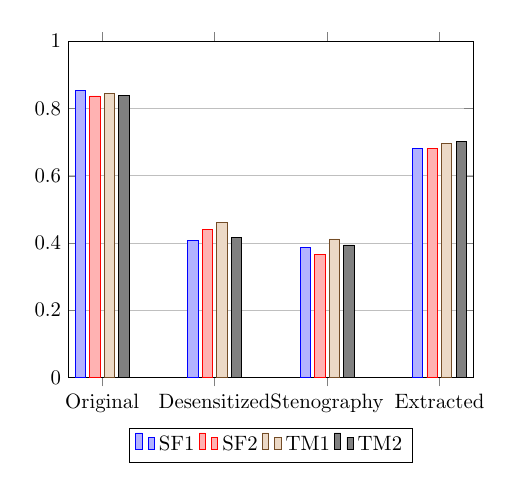
\begin{tikzpicture}[scale=0.75]
            \begin{axis}[
              ybar,
              bar width = 5pt,
              xtick = data,
              symbolic x coords = {Original, Desensitized, Stenography, Extracted},
              legend style={at={(0.5,-0.15)}, anchor=north,legend columns=-1},
              enlarge x limits = 0.1,
              ymajorgrids = true,
              ymin = 0,
              ymax = 1
            ]
            \addplot coordinates {
                (Original,0.853889)(Desensitized,0.407654)(Stenography,0.387695)(Extracted,0.681975)
            };
            \addplot coordinates {
                (Original,0.837284)(Desensitized,0.440206)(Stenography,0.366070)(Extracted,0.681728)
            };
            \addplot coordinates {
                (Original,0.84537)(Desensitized,0.460556)(Stenography,0.412119)(Extracted,0.695123)
            };
            \addplot coordinates {
                (Original,0.837963)(Desensitized,0.417078)(Stenography,0.394115)(Extracted,0.702593)
            };
            \legend{SF1,SF2,TM1,TM2}
            \end{axis}
          \end{tikzpicture}
    }
    \caption{Chart Of Mean Scores}
    \label{chart_mean}
\end{figure}

\begin{table}[!t]
    \centering
    \caption{Statistics of Differences Between Desensitized and Stenography Samples}
    \begin{tabular}{|c|c|}
        \hline
        \textbf{Mean} & 0.041373 \\
        \hline
        \textbf{Variance} & 0.010478 \\
        \hline
        \textbf{Maximum} & 0.37 \\
        \hline
        \textbf{Minimum} & -0.29 \\
        \hline
        \textbf{Maximum Absolute Value} & 0.37 \\
        \hline
        \textbf{Minimum Absolute Value} & 0 \\
        \hline
    \end{tabular}
\end{table}

\begin{figure}[!t]
    \centerline{
        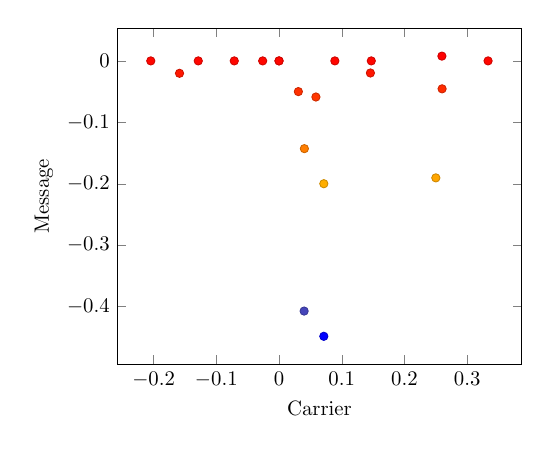
\begin{tikzpicture}[scale=0.75]\begin{axis}[xlabel={Carrier},ylabel={Message},]\addplot[scatter,only marks] coordinates {(0.1457,-0.0197)(-0.2045,0.0000)(0.0308,-0.0500)(0.0404,-0.1429)(0.0000,0.0000)(0.2500,-0.1905)(-0.1587,-0.0202)(-0.0261,0.0000)(0.3333,0.0000)(-0.0714,0.0000)(0.2597,0.0078)(0.1471,0.0000)(0.0890,0.0000)(0.0400,-0.4074)(-0.1288,0.0000)(0.0714,-0.4485)(0.2600,-0.0455)(0.0000,0.0000)(0.0714,-0.2000)(0.0588,-0.0588)};\end{axis}\end{tikzpicture}
    }
    \caption{Scatter of content degradation of all results, where \textit{Message} stands for the reduction of accuracy of the respective identity of each voice sequence from $x$ to $x^{\prime}$ and \textit{Carrier} from $y$ to $y^{\prime}$. Lower values are better and values below zero implies the improvement of accuracy.}
    \label{fig:degradation}
\end{figure}

\begin{figure}[!t]
    \centerline{
        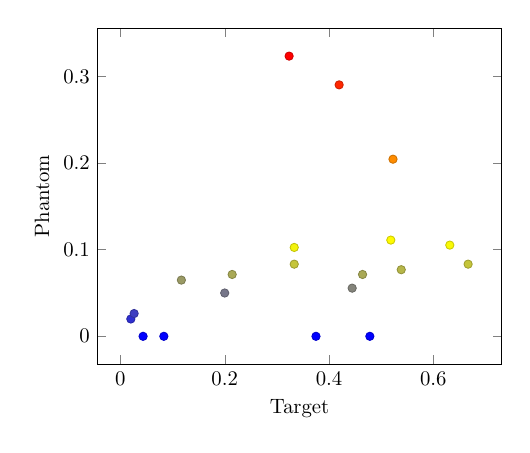
\begin{tikzpicture}[scale=0.75]\begin{axis}[xlabel={Target},ylabel={Phantom},]\addplot[scatter,only marks] coordinates {(0.1169,0.0649)(0.6316,0.1053)(0.2143,0.0714)(0.2000,0.0500)(0.3333,0.0833)(0.0833,0.0000)(0.3750,0.0000)(0.5385,0.0769)(0.6667,0.0833)(0.4643,0.0714)(0.4444,0.0556)(0.4194,0.2903)(0.5227,0.2045)(0.0200,0.0200)(0.4783,0.0000)(0.0435,0.0000)(0.3333,0.1026)(0.5185,0.1111)(0.0263,0.0263)(0.3235,0.3235)};\end{axis}\end{tikzpicture}
    }
    \caption{Scatter of conversion performance of results of $y$, where \textit{Phantom} means the accuracy of participant choosing the speaker of corresponding $x$ and \textit{Target} for the target speaker. Values closer to the right-bottom end are better.}
    \label{fig:transform}
\end{figure}

\begin{figure}[!t]
    \centerline{
        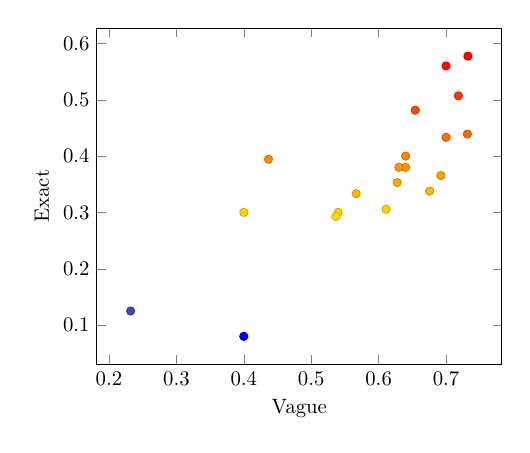
\begin{tikzpicture}[scale=0.75]\begin{axis}[xlabel={Vague},ylabel={Exact},]\addplot[scatter,only marks] coordinates {(0.7000,0.4333)(0.7183,0.5070)(0.6923,0.3654)(0.7000,0.5600)(0.4000,0.3000)(0.5400,0.3000)(0.6275,0.3529)(0.7317,0.4390)(0.5667,0.3333)(0.6757,0.3378)(0.5366,0.2927)(0.2321,0.1250)(0.6543,0.4815)(0.7324,0.5775)(0.6111,0.3056)(0.4366,0.3944)(0.6400,0.3800)(0.6300,0.3800)(0.4000,0.0800)(0.6400,0.4000)};\end{axis}\end{tikzpicture}
    }
    \caption{Scatter of gender recognition of all results, where \textit{Vague} is the accuracy of choosing a speaker that is of the same gender of the actual identity and \textit{Exact} is the accuracy of recognizing the exact speaker. Values closer to the right-bottom corner indicates a tendency of mixing up TM1, TM2 and SF1, SF2, where the gender of speakers are the same for each pair. }
    \label{fig:gender}
\end{figure}

\section{Future Work}
\label{seg:future}

In our experiment, we simply directed the voice sequence generated by the benign model to the stenography model. As mentioned before, this approach may not be sufficient in terms of stealthiness. Also, the overall storage consumption of this black box will increase significantly and the processing performance may not be ideal.

We believed that turning the stenography model into extra layers of benign model, eliminating the redundant audio encoding and decoding processes, can mitigate such problems while potentially increase the overall adversarial quality. In this way, the benign model can train in conjunction with the adversary model, taking advantage of intermediate representations of it. Moreover, this creates the potential of reducing the overall storage consumption and be less suspicious.

As another way to mitigate such problem, users can use various traditional or ML-based methods to apply inaudible perturbation on processed voices to attempt erasure of potential stenography while preserving high audio quality.

\section{Conclusion}
\label{seg:conclusion}

Targeting voice desensitization models based on generative NN models, we designed an adversary scheme that attempts to recover original voices from desensitized ones via stenography means, thus cause a privacy bleach. Our experiments prove this idea to be viable and the conventional solutions to be vulnerable to this type of adversary.

According to our experiments, it is safe to consider conventional acoustical-based or NN-based audio transforming solutions not sufficient for voice desensitization. Besides the StarGAN-VC solution we used, there exists many more such "voice changer" services on the Internet available for public use. One would consider these solutions secure because of the vast audible differences they made on its voice sequences. However, these solution exhibits potential of adversary with such method we demonstrated in this paper, which is not negligible. It's not likely that human ears can pick up subtle changes a stenography program made to certain parts of a voice sequence.

\begin{thebibliography}{00}
    \bibitem{a1} N. Subramanian, O. Elharrouss, S. Al-Maadeed and A. Bouridane, "Image Steganography: A Review of the Recent Advances," in IEEE Access, vol. 9, pp. 23409-23423, 2021, doi: 10.1109/ACCESS.2021.3053998.
    \bibitem{a3} Y. Li, X. Qiu, P. Cao, Y. Zhang, and B. Bao, “Non-parallel Voice Conversion Based on Perceptual Star Generative Adversarial Network,” Circuits Syst Signal Process, vol. 41, no. 8, pp. 4632–4648, Aug. 2022, doi: 10.1007/s00034-022-01998-5.
    \bibitem{a4} F. Kreuk, Y. Adi, B. Raj, R. Singh, and J. Keshet, “Hide and Speak: Towards Deep Neural Networks for Speech Steganography.” arXiv, Jul. 27, 2020. doi: 10.48550/arXiv.1902.03083.
    \bibitem{a5} N. Takahashi, M. K. Singh, and Y. Mitsufuji, “Source Mixing and Separation Robust Audio Steganography.” arXiv, Feb. 17, 2022. doi: 10.48550/arXiv.2110.05054.
    \bibitem{a6} Andreas Nautsch, Abelino Jiménez, Amos Treiber, Jascha Kolberg, Catherine Jasserand, Els Kindt, Héctor Delgado, Massimiliano Todisco, Mohamed Amine Hmani, Aymen Mtibaa, Mohammed Ahmed Abdelraheem, Alberto Abad, Francisco Teixeira, Driss Matrouf, Marta Gomez-Barrero, Dijana Petrovska-Delacrétaz, Gérard Chollet, Nicholas Evans, Thomas Schneider, Jean-François Bonastre, Bhiksha Raj, Isabel Trancoso, and Christoph Busch. 2019. Preserving privacy in speaker and speech characterisation. Comput. Speech Lang. 58, C (Nov 2019), 441–480. https://doi.org/10.1016/j.csl.2019.06.001
    \bibitem{a7} Kröger, J.L., Lutz, O.HM., Raschke, P. (2020). Privacy Implications of Voice and Speech Analysis – Information Disclosure by Inference. In: Friedewald, M., Önen, M., Lievens, E., Krenn, S., Fricker, S. (eds) Privacy and Identity Management. Data for Better Living: AI and Privacy. Privacy and Identity 2019. IFIP Advances in Information and Communication Technology(), vol 576. Springer, Cham.
    \bibitem{a8} Jaemin Lim, Kiyeon Kim, Hyunwoo Yu, and Suk-Bok Lee. 2022. Overo: Sharing Private Audio Recordings. In Proceedings of the 2022 ACM SIGSAC Conference on Computer and Communications Security (CCS '22). Association for Computing Machinery, New York, NY, USA, 1933–1946. https://doi.org/10.1145/3548606.3560572
    \bibitem{a9} J. Qian, H. Du, J. Hou, L. Chen, T. Jung and X. -Y. Li, "Speech Sanitizer: Speech Content Desensitization and Voice Anonymization," in IEEE Transactions on Dependable and Secure Computing, vol. 18, no. 6, pp. 2631-2642, 1 Nov.-Dec. 2021, doi: 10.1109/TDSC.2019.2960239.
    \bibitem{a10} Jianwei Qian, Haohua Du, Jiahui Hou, Linlin Chen, Taeho Jung, and Xiang-Yang Li. 2018. Hidebehind: Enjoy Voice Input with Voiceprint Unclonability and Anonymity. In Proceedings of the 16th ACM Conference on Embedded Networked Sensor Systems (SenSys '18). Association for Computing Machinery, New York, NY, USA, 82–94. https://doi.org/10.1145/3274783.3274855
    \bibitem{a11} J. Qian, F. Han, J. Hou, C. Zhang, Y. Wang and X. -Y. Li, "Towards Privacy-Preserving Speech Data Publishing," IEEE INFOCOM 2018 - IEEE Conference on Computer Communications, Honolulu, HI, USA, 2018, pp. 1079-1087, doi: 10.1109/INFOCOM.2018.8486250.
    \bibitem{a12} Nandwana, Mahesh Kumar, Julien van Hout, Mitchell McLaren, Allen R. Stauffer, Colleen Richey, Aaron D. Lawson and Martin Graciarena. “Robust Speaker Recognition from Distant Speech under Real Reverberant Environments Using Speaker Embeddings.” Interspeech (2018).
    \bibitem{a13} https://docs.aws.amazon.com/transcribe/latest/dg/pii-redaction.html
    \bibitem{a15} Audacity - Open source audio software. https://www.audacityteam.org/
    \bibitem{a16} T. Toda, L.-H. Chen, D. Saito, F. Villavicencio, M. Wester, Z. Wu, J. Yamagishi, "The Voice Conversion Challenge 2016," Proc. INTERSPEECH, pp. 1632-1636, 2016.
    \bibitem{a17} M. Wester, Z. Wu, J. Yamagishi, "Analysis of the Voice Conversion Challenge 2016 Evaluation Results," Proc. INTERSPEECH, pp. 1637-1641, 2016.
    \bibitem{a18} M. Wester, Z. Wu, J. Yamagishi, "Multidimensional scaling of systems in the Voice Conversion Challenge 2016," Proc. SSW9, pp. 40-45, 2016.
    \bibitem{pprl-vgan} J. Chen, J. Konrad, and P. Ishwar, “VGAN-Based Image Representation Learning for Privacy-Preserving Facial Expression Recognition,” in 2018 IEEE/CVF Conference on Computer Vision and Pattern Recognition Workshops (CVPRW), Salt Lake City, UT, USA, Jun. 2018, pp. 1651–165109. doi: 10.1109/CVPRW.2018.00207.
    \bibitem{subvert} K. Liu, B. Tan, and S. Garg, “Subverting Privacy-Preserving GANs: Hiding Secrets in Sanitized Images,” AAAI, vol. 35, no. 17, pp. 14849–14856, May 2021, doi: 10.1609/aaai.v35i17.17743.
\end{thebibliography}

\end{document}
